\section{Generating a phantom and a sinogram}

\begin{itemize}
\item Generate a phantom where each pixel consists of part bone and part water described as (bone, water)

\begin{itemize}
\item Background values should be low for both to simulate air (0, 0.05)
\item main body should be elliptical and mainly consist of water (0.20, 0.80)
\item elliptical inserts should simulate different organs and/or body featurs (0.80, 0.80)
\end{itemize}


\item Generate a sinogram from the projections

\begin{itemize}
\item The function will return a 3D object containing the sinograms for the height of the detector. We want to select a slice to display
\item print a 2D cross section of the phantom with a corresponding sinogram
\end{itemize}
\end{itemize}

\begin{verbatim}
#settings
objectSize = 32     # size of the object
nPixelsY = 64       # number of pixels in Y direction detector
nPixelsZ = 44       # number of pixels in Z direction detector
projections = 64   # number of projections
\end{verbatim}

\subsubsection{generate phantom}

\begin{verbatim}
import random, numpy as np

def generate_ct_matrices(n, h, num_features=5):

    # Initialize 3D bone and water matrices with zeros
    bone_matrix = np.zeros((n, n, n), dtype=float)
    water_matrix = np.zeros((n, n, n), dtype=float)

    # fill background of matrices with 0.05 bone and water 
    bone_matrix.fill(0)
    water_matrix.fill(0.05)
    
    # set values for main ellipse (simulated torso)
    intensity_bone = 0.2
    intensity_water = 0.8
    
    # Main body ellipse (simulated torso)
    for i in range(h, n - h):
        for j in range(2 * h, n - 2 * h):
            if ((i - n//2) / ((n - 2 * h) / 2)) ** 2 + ((j - n//2) / ((n - 6 * h) / 2)) ** 2 <= 1:
                
                bone_matrix[2*h: -2*h, i, j] = intensity_bone
                water_matrix[2*h: -2*h, i, j] = intensity_water

    # Adding smaller features (e.g., organs or bone structures)
    for _ in range(num_features):
        
        # Random place in the body - h is the offset from the edge, n is the size of the matrix
        a = random.randint(h, (n - h) // 4)  # Semi -major axis
        b = random.randint(h, (n - h) // 4)  # Semi -minor axis
        center_x = random.randint(h + a, n - h - a)
        center_y = random.randint(3 * h + b, n - 3 * h - b)

        # Randomly choose the intensity for bone and water, together they add to 1. 
        bone_intensity = 0.8
        water_intensity = 0.8
        
        for i in range(center_x - a, center_x + a):
            for j in range(center_y - b, center_y + b):
                if 0 <= i < n and 0 <= j < n:
                    if ((i - center_x) / a) ** 2 + ((j - center_y) / b) ** 2 <= 1:
                        bone_matrix[2*h: -2*h, i, j] = bone_intensity
                        water_matrix[2*h: -2*h, i, j] = water_intensity
    water_matrix *= 1  # Water density is 1
    bone_matrix *= 1.92  # Apply bone density
    
    return bone_matrix, water_matrix

bone, water = generate_ct_matrices(objectSize, 2, num_features=3)
x = np.column_stack((bone.ravel(), water.ravel()))
\end{verbatim}

\subsubsection{Running projection algorithm}

\begin{verbatim}
from libs.simulatepreps import projectMatrix

#generate proection matrices
y, S, M, A = projectMatrix(x, objectSize, nPixelsY, nPixelsZ, 1, projections)
\end{verbatim}

\subsubsection{Generating sinogram}

\begin{verbatim}
def getSinogram(y, energy_bin_index=0, z_index=32, nProj=100, detector_shape=(64, 44)):  
    nX, nZ = detector_shape
    y_bin = y[energy_bin_index]
    y_proj_zx = y_bin.reshape((nProj, nZ, nX))  # shape: (100, 64, 44)
    sinogram = y_proj_zx[:, z_index, :]  # shape: (100, 44)
    return sinogram

sinogram = getSinogram(y, energy_bin_index=0, z_index=objectSize // 2, nProj=projections, detector_shape=(nPixelsY, nPixelsZ))
\end{verbatim}

\subsubsection{Make figure}

\begin{verbatim}
import matplotlib.pyplot as plt


# plot bone density and phantom at objectSize //2 
plt.figure(figsize=(12, 6))
plt.subplot(1, 2, 1)
plt.imshow(bone[objectSize // 2, :, :], cmap='gray')
plt.title('Bone Density at z = {}'.format(objectSize // 2))
plt.xlabel('X')
plt.ylabel('Y')

plt.subplot(1, 2, 2)
plt.imshow(sinogram, cmap='gray')
plt.title('Sinogram at z = {}'.format(objectSize // 2))
plt.ylabel('Angle')
plt.xlabel('Y')

plt.tight_layout()
plt.show()
\end{verbatim}

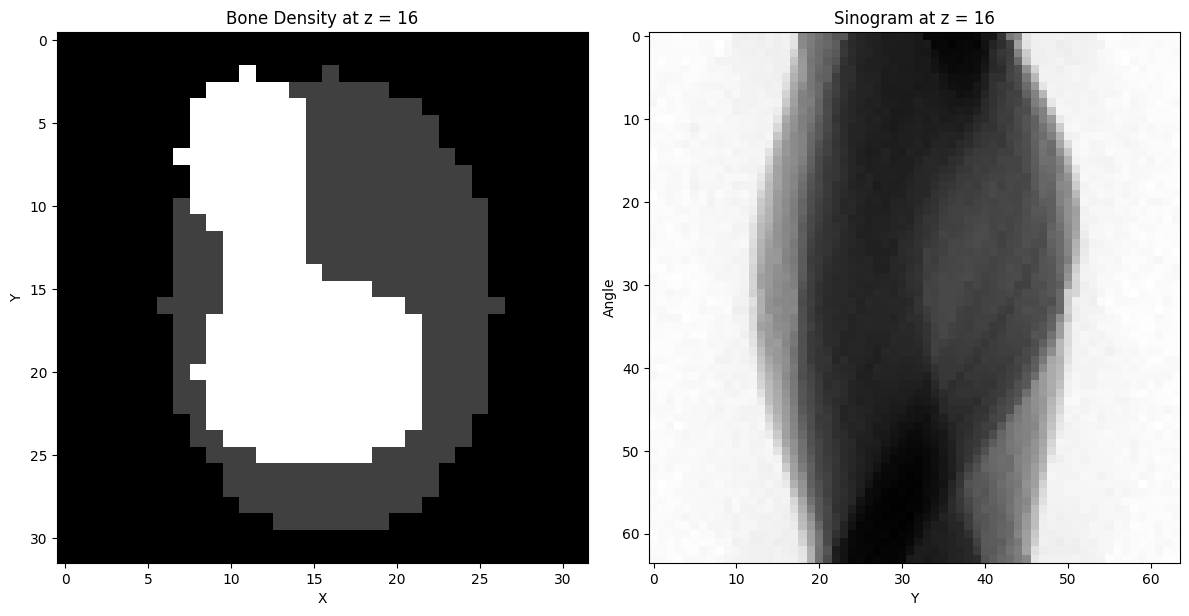
\includegraphics[width=0.7\linewidth]{files/b976b4c5294674aa189b37fdcfeb40f7.png}

\subsection{Visualising a 2D convolution}

\begin{verbatim}
# we want to put the phantom through a pytorch 2d convolution layer
import torch

bone_array = bone[objectSize // 2, :, :]
bone_tensor = torch.tensor(bone[objectSize // 2, :, :], dtype=torch.float32)

# create a 2D convolution layer with a kernel size of 3x3
conv_layer = torch.nn.Conv2d(in_channels=1, out_channels=1, kernel_size=3, padding=1)

# apply the convolution layer to the bone tensor
output_tensor = conv_layer(bone_tensor.unsqueeze(0).unsqueeze(0))  # Add batch and channel dimensions
output_image = output_tensor.squeeze(0).squeeze(0).detach().numpy()  # Remove batch and channel dimensions

# plot 2 plots, one of the original bone image with a square showing one of the convolution kernels, and next to it the output image
plt.figure(figsize=(12, 6))
plt.subplot(1, 2, 1)
plt.imshow(bone_tensor.numpy(), cmap='gray')
# draw a square representing the convolution kernel
kernel_size = conv_layer.kernel_size[0]
plt.gca().add_patch(plt.Rectangle((10.5, 20.5), kernel_size, kernel_size, edgecolor='red', facecolor='none', lw=2))
# fill square with rectengles for each pixel
for i in range(kernel_size):
    for j in range(kernel_size):
        plt.gca().add_patch(plt.Rectangle((10.5 + i, 20.5 + j), 1, 1, edgecolor='red', facecolor='none', lw=0.5))
plt.title('Original Bone Image at z = {}'.format(objectSize // 2))
plt.xlabel('X')
plt.ylabel('Y')
plt.subplot(1, 2, 2)
plt.imshow(output_image, cmap='gray')
# draw little square representing the pixel on which the convolution was applied
plt.gca().add_patch(plt.Rectangle((10.5+2, 20.5+2), 1, 1, edgecolor='red', facecolor='none', lw=2))
plt.title('Output Image after Convolution')
plt.xlabel('X')
plt.ylabel('Y')
\end{verbatim}

\begin{verbatim}
Text(0, 0.5, 'Y')
\end{verbatim}

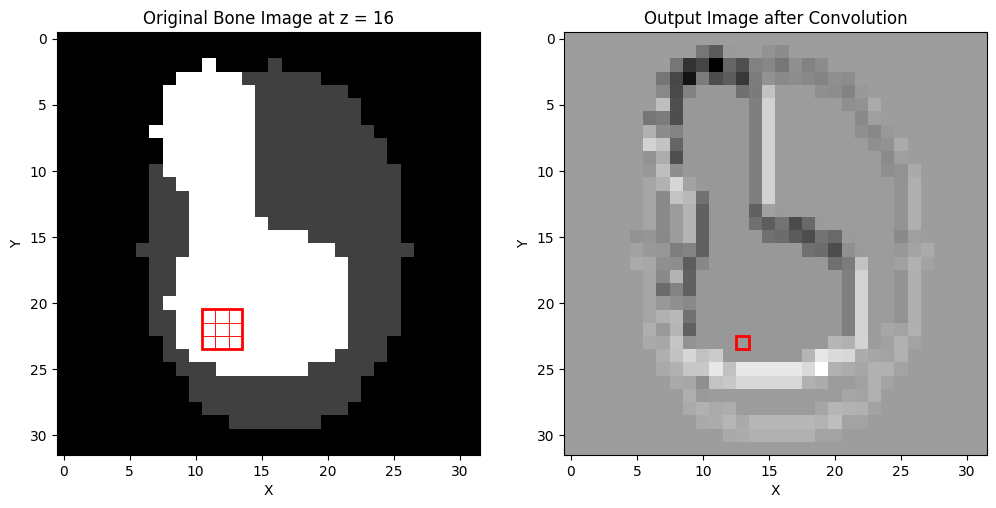
\includegraphics[width=0.7\linewidth]{files/53dfddea48d84244f37a3a2bae253fa3.png}